\chapter{Project description - extension}
This project description is an extension of the original project description made by Delta. It is made to clarify the borders and content of the bachelor project at the engineering college of Aarhus.\\
The description discards irrelevant subjects or elements of no interest. It adds new elements relevant for the students which is still in the range of the original project description.\\
The name of the project will be "Charcot foot prevention system".


\section{Background}
The original project description did not fulfil the demands to a bachelor project with regards to new technology and new knowledge. Therefore the original project description needs to be modified to accommodate the group and the supervisors requirements to a bachelors project. \\
This twist of the project has been made in collaboration with the project supervisor.\\
The extension includes new communication protocol development and smart-sensor development.\\
Therefore this project will lead more towards a conceptual development project than a real development project.\\


\section{Project description}
The new focus will be upon the temperature and accelerometer sensors and the development of a system with one or max two wires connecting the sensors. The sensors will be interconnected and connected to the Central data unit. Temperature sensors will be addressed by the Central data  unit. Data will be stored by the Central data unit for possible extraction by a user interface. \\

The main idea behind the temperature and accelerometer sensors points toward a prototype PCB with discrete components. The sensor board prototype board will be made on a large PCB with a simple layout to prove that the concept is possible. \\

For development purposes a grid line will be used to power the Central data unit. A development kit or board for the microprocessor or controller  will be used while developing the brain of the central data unit. \\

\section{Final Product}
\textit{The final product is out of our scope. For full understanding of the system the final product description is included in this section.}\\

The final product will entail a computer and a smart-phone to read data from the central data unit. They will also carry the alarms and messages from the system to the user. Further more it is possible to check the data history on these units. \\

The prototype sensor board is supposed to be made into an embedded IC which will be sealed with epoxy to fulfil the demand for hygiene and cleaning. The size of the embedded IC will also be small enough so that is does not interfere with the daily life of the user. The sensor IC will be placed in a sock for the user to wear. \\

The Central data collection unit will run on a rechargeable battery. This will allow the user to recharge the system over night and then use it during the day without being confined by grid wires.\\

Data can be extracted from the central data unit with a wireless protocol, a replaceable data card or with a USB protocol.
\begin{figure}[H]
\centering
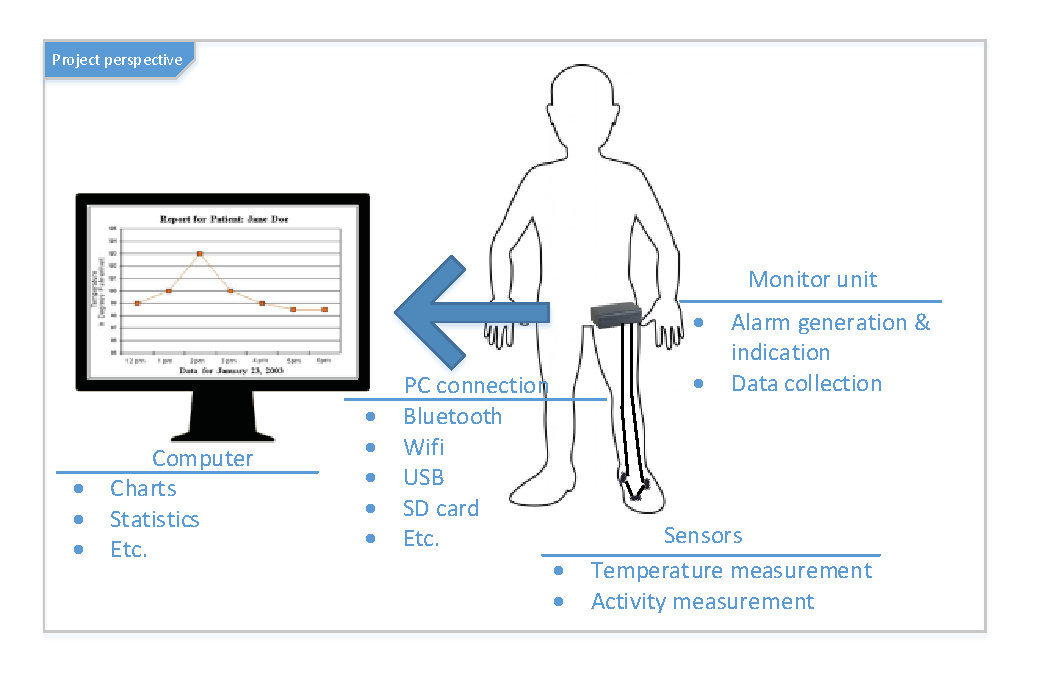
\includegraphics[width=0.8\textwidth]{billeder/fullsystem_vector}
\caption{The full system in perspective to the project.}
\end{figure}
